\section{Phần A: Kết quả thực nghiệm}
\label{sec:a-results}

\subsection{Thiết lập}

Mọi số liệu dưới đây dùng ngưỡng IoU $\ge 0.5$. Tham số và lựa chọn phương pháp được chọn trên tập tune (198 ảnh); các bảng chính báo trên tập test (462 ảnh) và chỉ đo cho cấu hình đã chốt. Các nhóm khó (\code{blur}, \code{db}, \code{challenge}, \code{tilt}) chỉ có 12 ảnh ở tune và 28 ảnh ở test, nên một ảnh đổi kết quả làm tỉ lệ thay đổi $1/28\approx 0.036$; chênh lệch nhỏ ở các nhóm này không nên đọc là xu hướng. Thời gian chạy (ms/ảnh) trong mục này và mục~\ref{sec:e7} đo trên một lần chạy một tiến trình, máy ít tải hơn so với các lần chạy ghi trong sổ thí nghiệm (khi đó nhiều tiến trình khác chạy cùng lúc, số tuyệt đối cao gấp khoảng ba lần); vì vậy chỉ nên so sánh tương đối giữa các dòng của cùng một bảng.

\subsection{Tiền xử lý: kích thước ảnh và bộ lọc nhiễu (E2)}
\label{sec:e2}

\textbf{Kích thước ảnh.} Ở giai đoạn đầu (tập tune, cấu hình định vị cũ), thử ba chiều rộng resize cho thấy ảnh càng lớn càng tốt (Bảng~\ref{tab:resize}); giữ 800.

\begin{table}[htbp]
\centering
\caption{Ảnh hưởng của chiều rộng resize (tune, $n=198$, cấu hình định vị giai đoạn đầu; nguồn: sổ thí nghiệm, mục Tiền xử lý).}
\label{tab:resize}
\small
\begin{tabular}{lrrrr}
\toprule
Chiều rộng & P & R & F1 & R@5 \\
\midrule
640 & 0.639 & 0.591 & 0.614 & 0.727 \\
720 (không đổi tỉ lệ) & 0.640 & 0.601 & 0.620 & 0.758 \\
\textbf{800 (chọn, phóng to)} & 0.647 & 0.621 & 0.634 & 0.778 \\
\bottomrule
\end{tabular}
\end{table}

\textbf{Bộ lọc nhiễu.} E2 chạy \code{localize\_edge} với bốn bộ lọc và cấu hình chốt của mục~\ref{sec:tuning}, trên cả tune và test (Bảng~\ref{tab:e2}). Bộ lọc được chọn chỉ theo F1 trên tune.

\begin{table}[htbp]
\centering
\caption{E2: bộ lọc nhiễu, \code{localize\_edge}, dòng ALL. Đậm là bộ lọc được chọn trên tune. Nguồn: \code{e2\_filters.csv}.}
\label{tab:e2}
\small
\begin{tabular}{llrrrrrr}
\toprule
Tập & Bộ lọc & $n$ & P & R & F1 & R@5 & ms/ảnh \\
\midrule
tune & \textbf{bilateral} & 198 & 0.775 & 0.748 & 0.761 & 0.828 & 132.5 \\
tune & gaussian & 198 & 0.630 & 0.601 & 0.615 & 0.682 & 95.0 \\
tune & median & 198 & 0.637 & 0.611 & 0.624 & 0.697 & 107.7 \\
tune & none & 198 & 0.598 & 0.571 & 0.584 & 0.657 & 97.4 \\
\midrule
test & \textbf{bilateral} & 462 & 0.729 & 0.682 & 0.705 & 0.792 & 111.1 \\
test & gaussian & 462 & 0.647 & 0.615 & 0.630 & 0.712 & 82.4 \\
test & median & 462 & 0.616 & 0.584 & 0.600 & 0.699 & 93.2 \\
test & none & 462 & 0.610 & 0.576 & 0.592 & 0.645 & 84.7 \\
\bottomrule
\end{tabular}

\end{table}

Bilateral cho F1 cao hơn rõ rệt trên cả hai tập: 0.761 so với 0.584--0.624 trên tune và 0.705 so với 0.592--0.630 trên test. Ba bộ lọc còn lại cho kết quả gần nhau, và trên test bộ lọc trung vị (0.600) chỉ nhỉnh hơn \code{none} (0.592) rất ít. Nguyên nhân có thể là bilateral làm mịn nhiễu và các chi tiết nền mà vẫn giữ cạnh nét ký tự, nên bản đồ cạnh Sobel ít ứng viên rác hơn (đây là giả thuyết, chưa kiểm tra riêng). Cái giá là thời gian: bilateral chậm hơn các bộ lọc khác khoảng 18--29 ms/ảnh trong lần đo này (111 ms so với 82--93 ms trên test). Nên dùng bilateral cho các thí nghiệm sau.

\subsection{Tinh chỉnh bước định vị trên tập tune}
\label{sec:tuning}

Cấu hình ban đầu (kernel close $17\times 3$, \code{fill\_ratio} tối thiểu 0.5, \code{edge\_density} tối thiểu 0.15) chỉ đạt Recall 0.348 trên tune. Quét từng tham số, mỗi lần đổi một hoặc hai tham số, cho thấy bước tăng lớn nhất là nới ngưỡng \code{fill\_ratio} và \code{edge\_density} (mặt nạ biển thật chỉ lấp khoảng 0.5 hình chữ nhật và mật độ cạnh khoảng 0.2), tiếp theo là chọn kernel close ngang rộng hơn (Bảng~\ref{tab:sweep}).

\begin{table}[htbp]
\centering
\caption{Một số dòng của đợt quét tham số định vị (tune, $n=198$, \code{localize\_edge}, top-1; \code{area\_ratio} $[0.002,0.10]$, chưa đa tỉ lệ). Nguồn: sổ thí nghiệm, mục Định vị.}
\label{tab:sweep}
\small
\begin{tabular}{lrrrr}
\toprule
Cấu hình & P & R & F1 & R@5 \\
\midrule
Mặc định cũ: close $[17,3]$, fill 0.5, dens 0.15 & 0.570 & 0.348 & 0.433 & 0.384 \\
fill 0.35, dens 0.10 (close $[17,3]$) & 0.545 & 0.515 & 0.530 & 0.682 \\
fill 0.35, dens 0.10 + close $[25,5]$ & 0.647 & 0.621 & 0.634 & 0.778 \\
fill 0.35, dens 0.10 + close $[21,5]$ & 0.672 & 0.641 & 0.656 & 0.783 \\
\textbf{close $[21,5]$, fill 0.40, dens 0.12 (chốt)} & \textbf{0.703} & \textbf{0.646} & \textbf{0.674} & \textbf{0.768} \\
\bottomrule
\end{tabular}
\end{table}

\textbf{Issue \#10: recall của ứng viên.} Sau đó chúng tôi nhận thấy biển thật thường bị bỏ sót vì vùng biển vỡ mảnh sau bước hình thái học, hoặc bị ứng viên nhỏ (logo, chữ) xếp trên. Tăng $k$ từ 5 lên 10 không đổi Recall, tức nút thắt nằm ở bộ lọc chứ không phải số ứng viên giữ lại. Top-1 sai thường là một vùng rất nhỏ (\code{area\_ratio} khoảng 0.002--0.003) trong khi biển thật có \code{area\_ratio} khoảng 0.015--0.05. Ba thay đổi được chọn trên tune: (i) thêm hai kernel close phụ và gộp bằng NMS, (ii) nâng cận dưới \code{area\_ratio} từ 0.002 lên 0.008 và cận trên từ 0.10 lên 0.16 theo phân bố bbox thật, (iii) nới \code{aspect} từ $[2,6]$ lên $[1.5,7]$ vì quad của vùng cạnh nghiêng hoặc dính viền dài/ngắn hơn biển thật. Bảng~\ref{tab:i10abl} cho thấy phần đóng góp của từng thay đổi trên tune; Bảng~\ref{tab:i10} so sánh trước và sau theo nhóm, đo trên test đúng một lần cho cấu hình chốt.

\begin{table}[htbp]
\centering
\caption{Issue \#10: đóng góp của từng thay đổi (tune, $n=198$, ALL, top-1). \code{cand\_recall} là Recall@5. Nguồn: sổ thí nghiệm, mục Issue \#10.}
\label{tab:i10abl}
\small
\begin{tabular}{lrrr}
\toprule
Cấu hình & \code{cand\_recall} & Recall@1 & P \\
\midrule
Cũ (close $[21,5]$, aspect $[2,6]$, area $[0.002,0.10]$) & 0.768 & 0.646 & 0.703 \\
Chỉ thêm hai kernel close $[13,3]$, $[33,7]$ & 0.828 & 0.652 & 0.665 \\
Chỉ đổi area thành $[0.008,0.16]$ & 0.753 & 0.712 & 0.829 \\
Area $[0.008,0.16]$ + hai kernel thêm & 0.818 & 0.747 & 0.787 \\
\textbf{+ aspect $[1.5,7.0]$ (chốt)} & \textbf{0.828} & \textbf{0.747} & \textbf{0.775} \\
\bottomrule
\end{tabular}
\end{table}

\begin{table}[htbp]
\centering
\caption{Issue \#10: cấu hình cũ $\to$ cấu hình chốt, tập test ($n=462$), \code{localize\_edge} (chưa SVM). Nguồn: sổ thí nghiệm, mục Issue \#10. Ở tune (ALL, $n=198$): \code{cand\_recall} $0.768\to 0.828$, Recall@1 $0.646\to 0.747$, P $0.703\to 0.775$.}
\label{tab:i10}
\small
\begin{tabular}{lrrrr}
\toprule
Nhóm & $n$ & \code{cand\_recall} & Recall@1 & P \\
\midrule
base & 350 & $0.729\to 0.874$ & $0.609\to 0.751$ & $0.644\to 0.771$ \\
blur & 28 & $0.500\to 0.643$ & $0.357\to 0.643$ & $0.400\to 0.750$ \\
challenge & 28 & $0.571\to 0.500$ & $0.429\to 0.464$ & $0.500\to 0.619$ \\
db & 28 & $0.464\to 0.429$ & $0.321\to 0.321$ & $0.409\to 0.409$ \\
tilt & 28 & $0.357\to 0.571$ & $0.286\to 0.429$ & $0.348\to 0.500$ \\
\midrule
ALL & 462 & $0.667\to 0.792$ & $0.545\to 0.682$ & $0.593\to 0.729$ \\
\bottomrule
\end{tabular}
\end{table}

Trên test, Recall@1 tăng từ 0.545 lên 0.682 và \code{cand\_recall} từ 0.667 lên 0.792, tức cải thiện không chỉ do khớp tune. Phần lớn lợi ích nằm ở nhóm \code{base} (Recall@1 $0.609\to 0.751$). Hai nhóm \code{db} và \code{challenge} gần như không đổi hoặc giảm nhẹ \code{cand\_recall} (với $n=28$ chỉ là 1--2 ảnh). Cái giá là thời gian: số ứng viên trung bình mỗi ảnh gần như không đổi nhưng thời gian tăng khoảng 40--50\% do thêm hai lượt hình thái học và tính đặc trưng (tune $309\to 426$ ms/ảnh, test $269\to 396$ ms/ảnh, đo khi máy đang tải nên chỉ mang tính tương đối). Có một trần cứng: bộ lọc diện tích dùng diện tích \code{minAreaRect}; trên test có 16/462 bbox thật có \code{area\_ratio} dưới 0.008 (nhỏ nhất 0.0032) và 1 bbox lớn hơn 0.16, nên những ảnh này bị loại ngay từ bước lọc.

\subsection{Định vị: so sánh \code{edge} và \code{edge\_svm} (E3)}
\label{sec:e3}

\textbf{Huấn luyện SVM.} Trên 792 patch của tune (198 dương, 594 âm), kiểm chứng chéo 5 fold cho accuracy $0.960\pm 0.006$, precision $0.922\pm 0.035$, recall $0.919\pm 0.041$, F1 $0.919\pm 0.013$ (trung bình $\pm$ độ lệch chuẩn giữa các fold). Con số này lạc quan vì chia theo patch (các patch của cùng một ảnh có thể rơi vào cả train lẫn validation) và vì mẫu âm ngẫu nhiên khá dễ; độ chính xác định vị thực tế thấp hơn nhiều (bên dưới).

\textbf{Kết quả.} E3 dùng bộ lọc bilateral (chọn ở E2). Phương pháp được chọn theo F1 ALL trên tune: \code{edge\_svm} (F1 0.818, so với 0.761 của \code{edge}). Bảng~\ref{tab:e3} và Hình~\ref{fig:e3} cho kết quả trên test.

\begin{table}[htbp]
\centering
\caption{E3: định vị theo nhóm, tập test, bộ lọc bilateral. Nguồn: \code{e3\_localization.csv}.}
\label{tab:e3}
\small
\begin{table}[htbp]
\centering
\caption[E3: định vị theo nhóm (test)]{E3: định vị theo nhóm, tập test, bộ lọc bilateral. Nguồn: \code{e3\_localization.csv}.}
\label{tab:e3}
\small
\rowcolors{2}{white}{tablerowalt}
\begin{tabular}{llrrrrrrr}
\toprule
\rowcolor{tableheader} \tblhd{Phương pháp} & \tblhd{Nhóm} & \tblhd{$n$} & \tblhd{P} & \tblhd{R} & \tblhd{F1} & \tblhd{R@1} & \tblhd{R@3} & \tblhd{R@5} \\
\midrule
edge & base & 350 & 0.771 & 0.751 & 0.761 & 0.751 & 0.871 & 0.874 \\
edge & blur & 28 & 0.750 & 0.643 & 0.692 & 0.643 & 0.643 & 0.643 \\
edge & challenge & 28 & 0.619 & 0.464 & 0.531 & 0.464 & 0.500 & 0.500 \\
edge & db & 28 & 0.409 & 0.321 & 0.360 & 0.321 & 0.429 & 0.429 \\
edge & tilt & 28 & 0.500 & 0.429 & 0.462 & 0.429 & 0.571 & 0.571 \\
edge & ALL & 462 & 0.729 & 0.682 & 0.705 & 0.682 & 0.790 & 0.792 \\
\midrule
edge\_svm & base & 350 & 0.856 & 0.834 & 0.845 & 0.834 & 0.874 & 0.874 \\
edge\_svm & blur & 28 & 0.667 & 0.571 & 0.615 & 0.571 & 0.643 & 0.643 \\
edge\_svm & challenge & 28 & 0.667 & 0.500 & 0.571 & 0.500 & 0.500 & 0.500 \\
edge\_svm & db & 28 & 0.500 & 0.393 & 0.440 & 0.393 & 0.429 & 0.429 \\
edge\_svm & tilt & 28 & 0.583 & 0.500 & 0.538 & 0.500 & 0.571 & 0.571 \\
edge\_svm & ALL & 462 & 0.803 & 0.751 & 0.776 & 0.751 & 0.792 & 0.792 \\
\bottomrule
\end{tabular}
\end{table}

\end{table}

\begin{figure}[htbp]
\centering
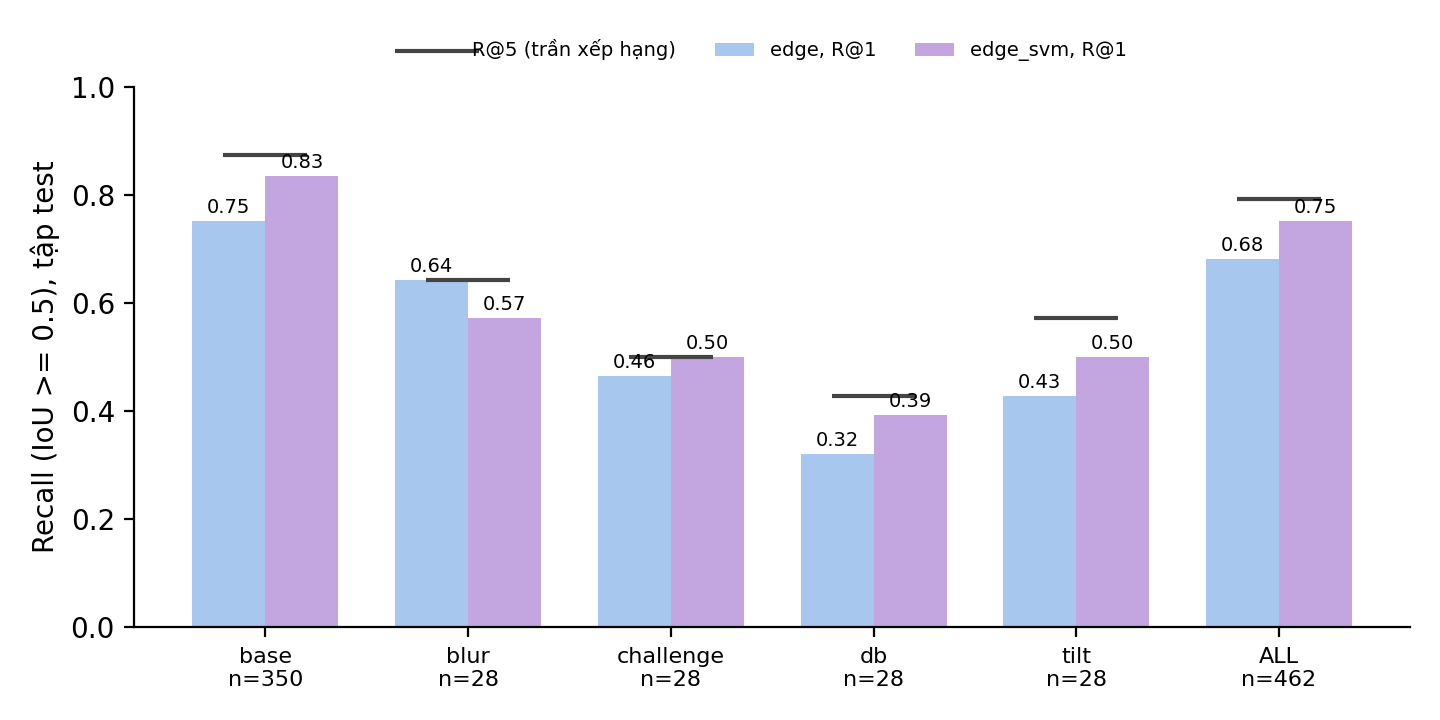
\includegraphics[width=0.85\textwidth]{figures/e3_subset_r1.png}
\caption{Recall@1 của \code{edge} và \code{edge\_svm} theo nhóm (test). Vạch đen là Recall@5, trần mà bước xếp hạng không vượt qua được. Nguồn: \code{e3\_localization.csv}.}
\label{fig:e3}
\end{figure}

Trên toàn test, top-1 của \code{edge\_svm} đạt $0.751$ so với $0.682$ của \code{edge} (tune: $0.803$ so với $0.747$; số tune của SVM lạc quan vì mô hình huấn luyện trên chính tập này). Mức tăng $+6.9$ điểm trên test tương ứng $+32$ ảnh trúng (315 $\to$ 347): \code{base} $+29$, \code{challenge} $+1$, \code{db} $+2$, \code{tilt} $+2$, \code{blur} $-2$. SVM không thêm ứng viên nên Recall@5 của hai phương pháp bằng nhau (0.792 trên test); toàn bộ cải thiện nằm ở Recall@1, và \code{edge\_svm} còn cách trần Recall@5 khoảng 4 điểm. Khoảng 21\% ảnh test không có ứng viên đúng trong top-5 (riêng \code{db} 57\%, \code{challenge} 50\%, \code{tilt} 43\%), nên muốn tăng tiếp thì phải cải thiện khâu sinh ứng viên, không phải khâu xếp hạng. SVM thêm 4.8 ms/ảnh trong E7 (sổ thí nghiệm ghi khoảng 14 ms khi máy đang tải).

\subsection{Nắn biển: cắt bbox so với warp quad (E4)}
\label{sec:e4}

E4 chạy toàn pipeline (định vị \code{edge\_svm} + bilateral, nhị phân Otsu, tách ký tự CCA của B) trên test, thay đổi duy nhất là cách lấy ảnh biển $220\times 70$: cắt bbox hay warp quad. Bảng~\ref{tab:e4} báo ba nguồn crop; Bảng~\ref{tab:e4sub} tách theo nhóm cho các ảnh top-1 đúng.

\begin{table}[htbp]
\centering
\caption{E4: cắt bbox so với warp quad, tập test, dòng ALL. Sai số góc tính theo pixel ảnh gốc trên 347 ảnh top-1 đúng. Nguồn: \code{e4\_rectify.csv}.}
\label{tab:e4}
\small
\resizebox{\textwidth}{!}{\begin{table}[htbp]
\centering
\caption[E4: cắt bbox so với warp quad (test, ALL)]{E4: cắt bbox so với warp quad, tập test, dòng ALL. Sai số góc tính theo pixel ảnh gốc trên 347 ảnh top-1 đúng. Nguồn: \code{e4\_rectify.csv}.}
\label{tab:e4}
\footnotesize
\setlength{\tabcolsep}{3pt}
\rowcolors{2}{white}{tablerowalt}
\arrayrulecolor{tableheader}
\begin{tabularx}{\textwidth}{llCCCCCC}
\hline
\rowcolor{tableheader} \tblhd{Nguồn crop} & \tblhd{Crop} & \tblhd{$n$} & \tblhd{corner (tb / trung vị)} & \tblhd{count\_\allowbreak match} & \tblhd{pos0} & \tblhd{pos1--6} & \tblhd{all\_\allowbreak correct} \\
\hline
gt & bbox & 462 & -- & 0.452 & 0.571 & 0.597 & 0.262 \\
gt & quad & 462 & -- & 0.606 & 0.805 & 0.815 & 0.563 \\
\hline
pred & bbox & 462 & 25.2 / 19.4 & 0.262 & 0.266 & 0.391 & 0.093 \\
pred & quad & 462 & 16.3 / 13.8 & 0.400 & 0.496 & 0.518 & 0.195 \\
\hline
pred\_tp & bbox & 347 & 25.2 / 19.4 & 0.346 & 0.329 & 0.498 & 0.124 \\
pred\_tp & quad & 347 & 16.3 / 13.8 & 0.513 & 0.625 & 0.641 & 0.259 \\
\hline
\end{tabularx}
\end{table}
}
\end{table}

\begin{table}[htbp]
\centering
\caption{E4 theo nhóm, chỉ ảnh top-1 đúng (\code{pred\_tp}), tập test. \code{corner}: sai số góc trung bình (px); \code{count}: \code{count\_match}; \code{all}: \code{all\_correct}. Nguồn: \code{e4\_rectify.csv}.}
\label{tab:e4sub}
\small
\resizebox{\textwidth}{!}{\begin{tabular}{lrrrrrrr}
\toprule
Nhóm & $n$ & corner bbox & corner quad & count bbox & count quad & all bbox & all quad \\
\midrule
base & 292 & 23.0 & 15.3 & 0.387 & 0.558 & 0.130 & 0.291 \\
blur & 16 & 22.8 & 16.0 & 0.125 & 0.062 & 0.125 & 0.000 \\
challenge & 14 & 23.7 & 19.2 & 0.143 & 0.214 & 0.000 & 0.143 \\
db & 11 & 34.7 & 24.0 & 0.273 & 0.455 & 0.273 & 0.273 \\
tilt & 14 & 68.0 & 28.9 & 0.000 & 0.429 & 0.000 & 0.000 \\
ALL & 347 & 25.2 & 16.3 & 0.346 & 0.513 & 0.124 & 0.259 \\
\bottomrule
\end{tabular}
}
\end{table}

Warp quad thắng cắt bbox ở mọi cột trên ALL: sai số góc giảm từ $25.2$ xuống $16.3$ px (trung vị $19.4\to 13.8$), \code{all\_correct} trên các ảnh top-1 đúng tăng từ $0.124$ lên $0.259$. Khi cô lập hẳn khỏi lỗi định vị (crop \code{gt}), \code{all\_correct} tăng từ $0.262$ lên $0.563$, tức phép nắn tự nó đã làm chất lượng tách ký tự tăng hơn gấp đôi tách ký tự. Nhóm \code{tilt} cho thấy đúng lý do: bbox ngang không bù được độ nghiêng, sai số góc $68.0$ px so với $28.9$ px của quad và \code{count\_match} $0.000$ so với $0.429$.

\textbf{Ngoại lệ ở nhóm \code{blur}} ($n=16$ ảnh top-1 đúng): bbox nhỉnh hơn quad ở \code{all\_correct} ($0.125$ so với $0.000$), \code{count\_match} ($0.125$ so với $0.063$) và \code{pos1--6} ($0.240$ so với $0.229$), dù sai số góc của quad vẫn tốt hơn ($16.0$ so với $22.8$ px). Chênh lệch này là 1--2 ảnh (một ảnh bằng $0.063$) nên chưa kết luận được. Nhóm \code{tilt} hòa ở \code{all\_correct} (cùng bằng 0) vì cả hai cách đều hỏng hết.

Có hai cảnh báo. Thứ nhất, lợi ích của \code{approxpoly} so với \code{minarearect} nhỏ: trên 128 ảnh tune có top-1 đúng (cấu hình định vị giai đoạn đầu), sai số góc trung bình chỉ giảm từ $19.7$ xuống $17.6$ px; theo từng ảnh có 45 ảnh tốt hơn, 48 kém hơn, 35 hòa (Wilcoxon $p=0.46$), nên khác biệt này không có ý nghĩa thống kê, và hằng số được chỉnh trên đúng tập đó. Lợi ích lớn ở E4 chủ yếu đến từ việc dùng quad nghiêng thay vì bbox ngang. Thứ hai, ở crop \code{gt} và \code{pred\_tp} có khoảng cách lớn ($0.563$ so với $0.259$ ở \code{all\_correct} của warp quad): dù IoU $\ge 0.5$, quad dự đoán vẫn lệch trung bình khoảng 16 px so với quad thật, đủ làm hỏng khoảng một nửa số biển ở bước tách ký tự. Trong 128 ảnh tune nói trên, 107 ảnh có ít nhất một góc thật nằm ngoài quad ứng viên, nên trần sai số do bước định vị quyết định, không phải bước tinh chỉnh quad.

\subsection{Thời gian chạy từng bước (E7)}
\label{sec:e7}

E7 đo thời gian từng bước của pipeline đầy đủ trên test (Bảng~\ref{tab:e7}), một tiến trình, ms/ảnh.

\begin{table}[htbp]
\centering
\caption{E7: thời gian từng bước, tập test, dòng ALL (ms/ảnh). Nguồn: \code{e7\_runtime.csv}. Bước ``Sobel, morph, lọc, NMS'' được ước lượng bằng hiệu thời gian \code{localize\_edge} trừ thời gian tiền xử lý đo riêng. 30 ảnh không có ứng viên nên các bước sau định vị chỉ có $n=432$.}
\label{tab:e7}
\small
\begin{table}[htbp]
\centering
\caption[E7: thời gian từng bước (test, ALL)]{E7: thời gian từng bước, tập test, dòng ALL (ms/ảnh). Nguồn: \code{e7\_runtime.csv}. Bước ``Sobel, morph, lọc, NMS'' được ước lượng bằng hiệu thời gian \code{localize\_edge} trừ thời gian tiền xử lý đo riêng. 30 ảnh không có ứng viên nên các bước sau định vị chỉ có $n=432$.}
\label{tab:e7}
\small
\rowcolors{2}{white}{tablerowalt}
\arrayrulecolor{tableheader}
\begin{tabularx}{\textwidth}{lCCC}
\hline
\rowcolor{tableheader} \tblhd{Bước} & \tblhd{$n$} & \tblhd{tb (ms)} & \tblhd{p95 (ms)} \\
\hline
tiền xử lý (resize, xám, CLAHE, lọc) & 462 & 69.79 & 134.32 \\
Sobel, morph đa tỉ lệ, lọc, NMS (ước lượng) & 462 & 63.50 & 149.30 \\
HOG + SVM & 462 & 4.77 & 10.77 \\
ước lượng quad & 432 & 0.97 & 2.20 \\
warp 220$\times$70 & 432 & 0.34 & 0.59 \\
nhị phân hóa (B) & 432 & 0.10 & 0.18 \\
tách ký tự (B) & 432 & 0.43 & 0.76 \\
\hline
\textbf{tổng (không SVM)} & 462 & 135.01 & 247.69 \\
\textbf{tổng} & 462 & 139.79 & 262.16 \\
\hline
\end{tabularx}
\end{table}

\end{table}

Tổng thời gian trung bình là 139.8 ms/ảnh (p95 262.2 ms). Định vị chiếm gần như toàn bộ: tiền xử lý khoảng 50\% (69.8 ms, phần lớn là bilateral đường kính 11 trên ảnh 800 px), Sobel cùng morph đa tỉ lệ khoảng 45\% (63.5 ms), SVM khoảng 3\% (4.8 ms). Các bước nắn, nhị phân hóa và tách ký tự cộng lại chỉ 1.8 ms. Theo nhóm, \code{tilt} chậm nhất (208.4 ms) và \code{challenge} nhanh nhất (88.5 ms; \code{db} 92.6 ms). Số tuyệt đối trong lần đo ghi trong sổ thí nghiệm cao hơn nhiều (416 ms/ảnh) vì máy khi đó đang chạy nhiều tiến trình; tỉ lệ giữa các bước ổn định hơn (tiền xử lý 44\%, SVM 3.3\%). Nếu cần số tuyệt đối cho kết luận về tốc độ thì nên đo lại trên máy riêng.
